\documentclass[aps,
                pra,  
                a4paper, 
                amsmath, 
                amssymb, 
                preprint,
                %tightenlines,  
                amsfonts,
                nofootinbib,
                %onecolumn,
                titlepage
            ]{revtex4-2}
\usepackage[utf8]{inputenc}
\usepackage{geometry, amsmath, amsthm, latexsym, amssymb, graphicx, amsfonts}

\begin{document}

%\title{Improving the optomechanics of a BAW resonator for quantum amplification within future gravitational wave detectors}
%\author{Joseph Hocking\\\textbf{Supervisors:} Prof. C. Zhao, Prof. Ju Li}
%\noaffiliation
%\date{\today}

\begin{titlepage}
    \begin{center}
        %\vspace*{1cm}
            
        \Large
        \textbf{Improving the optomechanics of a BAW resonator for quantum amplification within future gravitational wave detectors}
            
        %\vspace{0.5cm}
        %\LARGE
        %Thesis Subtitle
            
        \vspace{1.5cm}
        
        \large
        \textbf{Joseph Hocking}\\
        \vspace{0.25cm}
        \textbf{Supervisors:} Prof. C. Zhao, Prof. Ju Li
            
        \vfill
            
        A Research Proposal for the degree of\\
        Master's in Experimental Physics
            
        \vspace{0.8cm}
            
        
\includegraphics[width=0.4\textwidth]{img/uwa-logo.png}
            
        \large
        ARC Centre of Excellence for Gravitational Wave Discovery\\
        Department of Physics\\
        University of Western Australia\\
        \today
            
    \end{center}
\end{titlepage}

\section{Introduction}
    \par
    Gravitational waves, ripples in the very fabric of space-time, were once thought to be the playground of theoretical physicists. A fun quirk falling out of Einstein's revolutionary theory of general relativity. That was until in September of 2015, when we first directly heard the rumblings of universe. A true testament to the hard work and utter dedication of over half a century of international collaboration. We are now on the cusp of a new era of astronomy, the era of gravitational wave detection. It was Feynman, in a conference in 1957, described the first gravitational wave detector (GWD) in a mock thought experiment. Imagine a rigid rod, with two beads freely sliding (with friction), as the gravity wave passes through the rod the rigidity of it does not allow it to move with the wave. However, the proper distance between the beads will move, and due to this some small amount of energy will be deposited within the system, energy from the wave itself. Thus a it was realised that, theoretically at the minimum, one could detect gravitational waves. It was quickly noted, however, that due to the incredible stiffness of space-time, there existed no such material that could resist the motion of the wave.
    \par
    The first experimental attempts at gravitational wave detections were through the use of \textit{Resonant Mass Antennas}. These, as shown in Figure \ref{pic:resonant_bar}, consist of a large bar precisely machine to have a resonant frequency matching that of expected gravitional wave sources. These achieved sensitivies on the order of $10^{-19}\varepsilon/\sqrt{Hz}$, chiefly through the use of advanced seismic isolation systems, cryogenic cooling, and materials with extreme mechanical Q-factors. There were some who claimed (and some who still do) that these incredible experimental system did detect gravitional waves, see ref{ref:webber-detection}, but the consensus of the wider scientific community beleives that there simply were not sensitive enough.
    \begin{figure}
        \centering
        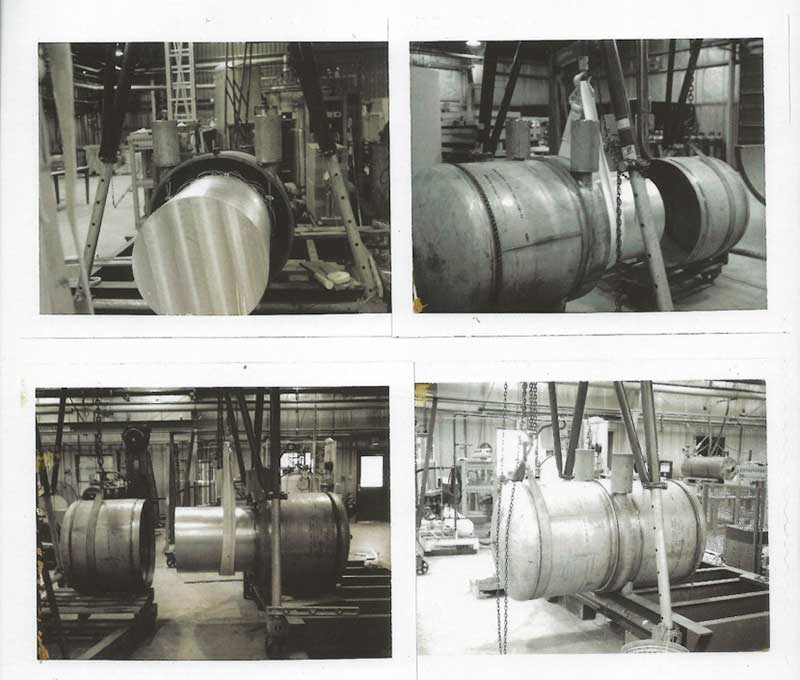
\includegraphics[width=0.5\textwidth]{img/weber-bar.jpg}
        \label{pic:resonant_bar}
    \end{figure}
    \par
    % TODO WIP Section. Need clear explanation of GWDs}\\
    The next, and current, generation of GWDs came in the form of large laser-based interferometers. A high powered, usually 1064nm, laser is split down two arms, which have a mirror at their respective ends. The photons, upon returning destructively interfere at the output port. When a GW signal couples into the detector, one of the arms are slightly elongated, meaning that there ius no longer complete destructive interference and the signal is detected. This is a huge over simplification of the system but for the purposes of this proposal, it will suffice to illustrate the point. 

\section{Quantum Amplification through White Light cavities}
    \subsection{Gravitational Wave Detector Noise}
    \label{sec:gwd-noise}
    % TODO add gwd noise curve
    For gravitational wave instrumentation, one of the most important figures is the interferometer noise curve, shown in ref{fig:noise-curve}. It is a measure of the minimum amplitude detectable by any given GWD, and can be seperated into several sources of noise. Within the low frequency regime, we become limited by the seismic motion of the ground the detector is situated upon. Then within the 10-20Hz range we begin to see the thermal noise of the suspension system spike. However, soon after that going all the way up to ~100Hz we are limited by radiation pressure noise. As the photons are reflected off the suspended mirrors, an imperceptible force is exterted, but due to the extreme laser powers and sensitivities, this small force is enough to push the mirror and produce noise within this frequency band. Beyond this, is where the research within this proposal focuses upon. In this high frequency band (1kHz) we are dominated by quantum shot noise. Due the Poisson counting statistics of the photons, the quantum shot noise is inversely proportional to the square root of the number of photons. In low frequency detections, when we have many photons hitting a photodetector, this variation is negligible, but at the high frequencies of the GW we no longer have the same power level, so this noise is dominates. 
    \par
    Fundamentally, this shot noise is dictated by the Quality factor of the optical resonators implemented within the GWD. Traditionally all resonators follow a \textit{gain-bandwidth relationship} where, for a given resonator design, we must maintain a fixed gain-bandwidth product, that is, if we wish to increase our gain, we must decrease our bandwidth. Within current generation GWDs, we must design resonators that strike a fine balance in this relationship. There is a strong need for high gain, as this increases photon lifetime within the arm cavity, and thus increasing the coupling of the gravitational wave into the detector. This however, necessarily reduces the detection bandwidth, limiting the amount of information we can extract from the signal (that is, introduces shot noise at higher frequencies).  
    \subsection{White Light Cavities}
    In 1997, Whicht et al. proposed a scheme, from here referred to as a White Light Cavity or WLC, to utilize a quantum mechanics to break this gain-bandwidth relationship. As a photon couples to a gravitational wave, its frequency, and thus accumulated phase, is red and blue shifted by the gravitational wave. This frequency shift results in a small difference in the accumulated phase of the photon, which increases the longer the photon lifetime within the cavity is. The proposed scheme would introduce a medium into the signal recycling cavity that would correct the phase, whilst maintaining the frequency shift induced by the gravitational wave. The corrected photons would then be fed back into the arm cavities for further amplification. Such a medium would be said to have an anomalous (also called negative) dispersion effect (AD or ND), that is the phase shift would be inversely proportional to frequency. This would, in effect, widen the bandwidth of the arm cavities whilst maintaining the same high gain. Mathematically, for carrier laser frequency $\omega_0$, the detectors arm length, $L_{arm}$, is tuned such that
    \begin{equation}
        \label{eq:cavity-resonance-condition}
        \frac{\omega_0L_{arm}}{c} = n\pi, \qquad n\in\mathbb{Z}
    \end{equation}
    When a gravitational wave of frequency $\Omega$ couples into the detector, our signal now has a frequency $\omega_0+\Omega$, these photons will therefore experience a phase shift of $\phi_{shift}=2\Omega L_{arm}/c$. So ideally, our negative dispersion medium will have a frequency dependent phase shift of
    \begin{equation}
        \label{eq:phase-correction}
        \phi_{ND} = -\frac{2\Omega L_{arm}}{c}
    \end{equation}
    % TODO Add figure of the acc. phase and phase correction here
    Along with their proposal for the WLC scheme, Whicht et al. suggested that an atomic media may create a sufficient negative dispersion effect, however it was later shown that, when implemented into a interferometric system, optical instability would place unrealistic constraints on the media, making it unsuitable for use within a WLC scheme. An alternative proposed method of inducing negative dispersion is through the use of an unstable optomechanical filter, this has been the focus of WLC research as of recently. There are three candidate optomechanical resonators (that may be used to create the unstable filter):
    \begin{description}
        \item[Phononic Membrane] This is a small mebrane made from a highly reflective crystal, which a lattice of holes punched into the surface such that they create a mechanical band gap that traps phonons within a defect in the lattice. This benefits from low mass and high mechanical Q factor, but suffers from large thermal heating due to its small heat capacity.
        \item[Catflap Resonator] % TODO Add description of Catflap resoantor
        \item[Bulk Acoustic Wave (BAW) Resonator] This is the focus of this proposal, and will be explained in detail further on, but as a brief description: The BAW is a plano-convex quartz crystal that is able to form a bulk phonon wave, this allows for a large mechanical Q, and its relatively large mass is beneficial for reducing the effect of laser heating. The large mass, on the other hand, also results in low optomechanical coupling, requiring large amounts of laser power for sufficient negative dispersion to occur.
    \end{description}
    
    \subsection{Overview of ND through Optomechanical Resonators}
    For any optomechanical interaction, we may model it through a 3-mode interaction, which have an input-output relation of
    \begin{equation}
        \label{eq:3-mode-in-out}
        \hat{a}_{out}=\frac{\Omega+i(\gamma_m+\gamma_{opt})}{\Omega+i(\gamma_m-\gamma_{opt})}\hat{a}_{in} + \hat{n}_{th}
    \end{equation}
    Where our mechanical damping is given by $\gamma_m\equiv\omega_m/Q_m$, with $Q_m$ being the mechanical Q factor of our optomechanical filter. And our negative optomechanical damping is given by $\gamma_{opt}\approx P_c\mathcal{F}\omega_0/(m\omega_m c^2)$, where $P_c$ is the intracavity power with the signal recycler, $\mathcal{F}$ is the cavity finesse, $m$ is the mass of the optomechanical resonator with resonant frequency $\omega_m$. Included in this equation is the thermal noise term, $\hat{n}_{th}$, this will be ignored for now but will place further requirements on the resonator. Note that this only applies within the resolved sideband regime, that is, when $\omega_m\gg\gamma_f\gg\Omega$, for filter cavity bandwidth $\gamma_f$. Additionally, by operating as an unstable optomechanical filter, which by definition is the regime such that $\gamma_{opt}\gg\gamma_m$, we can make the following approximations
    \begin{equation}
        \label{eq:in-out-approx}
        \hat{a}_{out}\approx\frac{\Omega+i\gamma_{opt}}{\Omega-i\gamma_{opt}}\hat{a}_{in}\approx-\exp{\left(\frac{-2i\Omega}{\gamma_{opt}}\right)}\hat{a}_{in}
    \end{equation}
    That is, our output experiences a phase shift of $\phi=-2\Omega/\gamma_{opt}$, so to satisfy the requirements outlined in Eqn \eqref{eq:phase-correction}, we have
    \begin{align}
        \label{eq:gamma-opt-req}
        \gamma_{opt}&=\frac{2\Omega L_{arm}}{c}\approx\frac{P_c\mathcal{F}\omega_0}{m\omega_m c^2}\\
        \label{eq:filter-power-req}
        \implies P_c&=2\frac{m\omega_m c \Omega L_{arm}}{\mathcal{F}\omega_0}
    \end{align}
    \par
    Additionally, we can examine the restrictions placed on the mechanical Q-factor of the resonator, $Q_m$, through the effect of thermal noise. $\hat{n}_{th}$ is uncorrelated with the input optical field % TODO need much more clarification upon this!!!!
    So that the effect does not dominate over any benefit from the WLC scheme, we require that
    \begin{equation}
        \label{eq:thermal-noise}
        \frac{8k_BT_{envir}}{Q_m}<\hbar\gamma_{IFO}
    \end{equation}
    %TODO Add figure of strain sensitivity at different T/Q
    Where $\gamma_{IFO}$ is the detector bandwidth prior to the implementation of the unstable filter, and $T_{envir}$ is the resonator temperature. This provides a convient figure of merit for optomechanical filters to be used in the WLC scheme, $T/Q$. As an order of magnitude estimate, to maintain near the sensitivities of current generation interferometers, we require $T/Q\sim10^{-10}K$. That is, if we operate our mechanical filter at 1K, we would require a mechanical Q factor of $10^{10}$. 
    


\end{document}